\newpage
\section{Versuchsdurchführung}
Der Versuch wurde entsprechend der Anweisungen aus der Laboranleitung \cite{Laboranleitung} durchgeführt.
Zu Beginn wird unter Anleitung und Erklärung der Laborleitung Fr. Kupzok die
Funktionalität der Anlage geprüft und sichergestellt, so dass die Anlage und Komponenten korrekt angeschlossen sind.\\
Die erste Messung hat das Ziel den Generatorwirkungsgrad beider PV-Generatoren im Aufbau 2 (DC-Betrieb) zu bestimmen.
Zusätzlich wird jeweils eine PV-Kennlinie aufzuzeichnen. Hierfür wird die benötigte Messtechnik angeschlossen und ein verstellbarer Widerstand verschaltet.
Während der Versuche wird die Bestrahlungsstärke mit einem Pyranometer gemessen.\\
\begin{figure}[!ht]
		\centering
		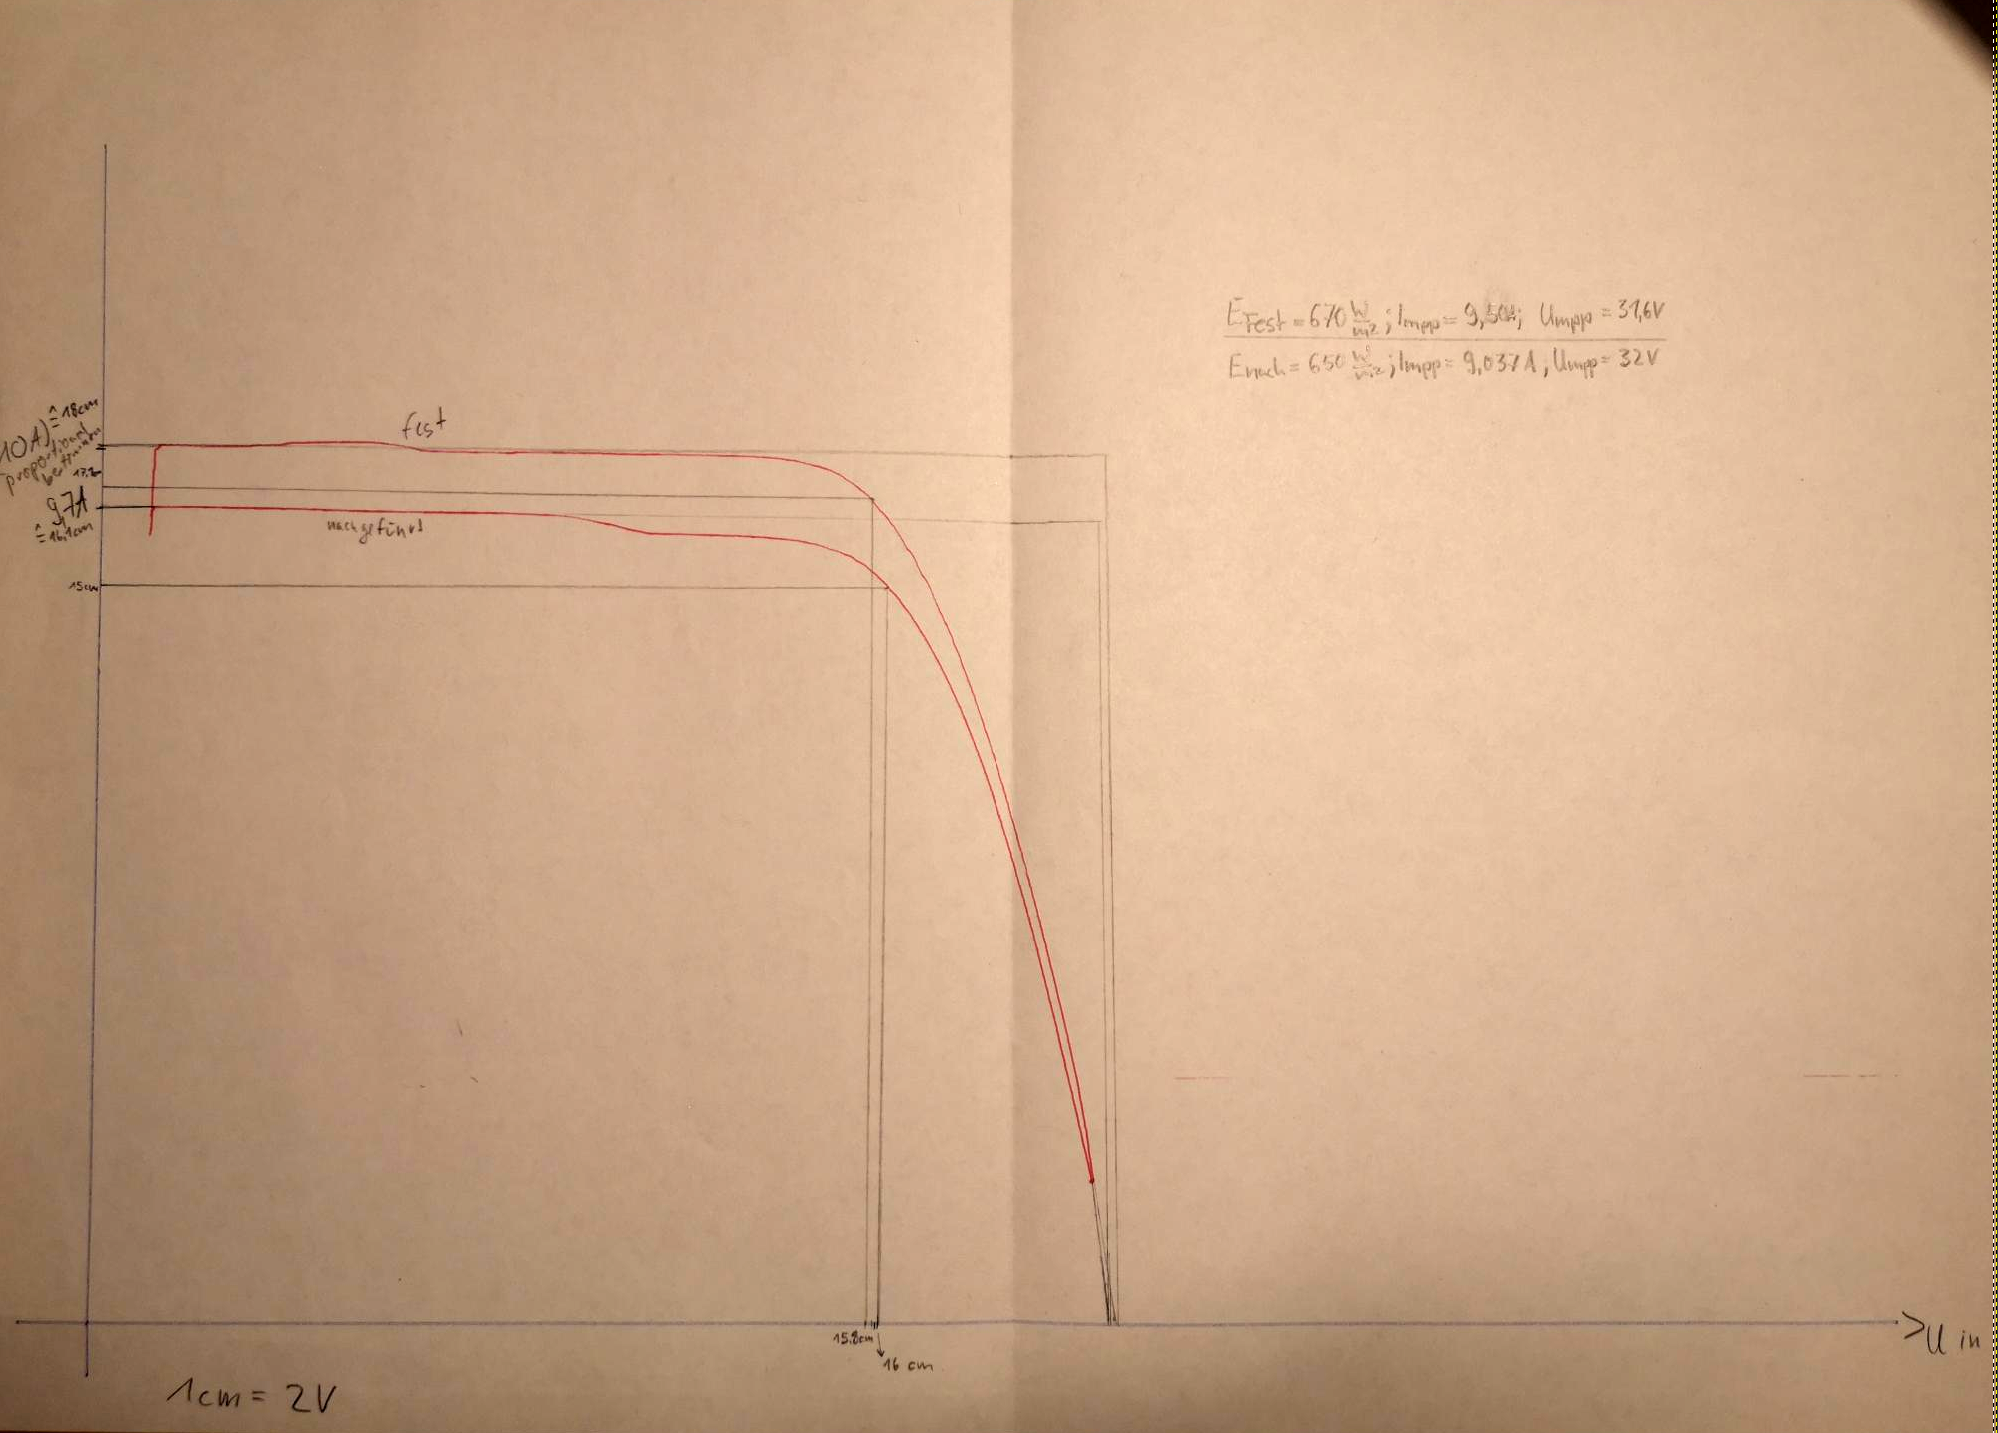
\includegraphics[width=0.7\textwidth]{Abbildungen/Kennlinie_PVGEN}
		\caption{Kennlinie des PV-Generators in Abhängigkeit von der Bestrahlungsstärke}
		\label{fig:230514_PVGEN_Kennlinie}
\end{figure}

Mittels des verstellbaren Widerstandes wird das System in den Leerlauf geführt und dann die Leerlaufspannung bestimmt.
Durch das Überbrücken des Widerstandes wird der Kurzschlussfall herbeigeführt und der Kurzschlusstrom gemessen.\\
Im zweiten Teil des Versuches wird Aufbau 1 verwendet, welcher den AC-Betrieb ermöglicht.
Ziel des zweiten Teils ist die Ermittlung der in der Anleitung \cite[S.8]{Laboranleitung} aufgeführten Kennwerte.\\
Hierzu gehören die Umgebungstemperatur, Bestrahlungsstärke, sowie Spannungen und Ströme an den relevanten Komponenten.
Zusätzlich wird auch der zeitliche Spannungsverlauf des Wechselrichters auf der AC-Seite mit einem Oszillogramm aufgenommen.
Diese Kennwerte wird für die folgenden Belastungsfälle bestimmt:
\begin{itemize}
    \item Ohne Last, nur der Wechselrichter ist in Betrieb
    \item geringe Ohmsche-induktive Last, Staubsauger Stufe 1
    \item mittlere Ohmsche-induktive Last, Staubsauger Stufe 2
    \item hohe Ohmsche-induktive Last, Staubsauger Stufe 3
    \item rein Ohmsche Last, S-Bahn-Heizung
\end{itemize}